

\begin{exercise}{Digitalisierung von analogen Signalen }
\label{ex-de-mt-gestaltprinzipien}
Gegeben sei folgendes periodisches Sinussignal:
$f(x)=sin(0.5\pi x)+sin(\pi x)+sin(2\pi x)$

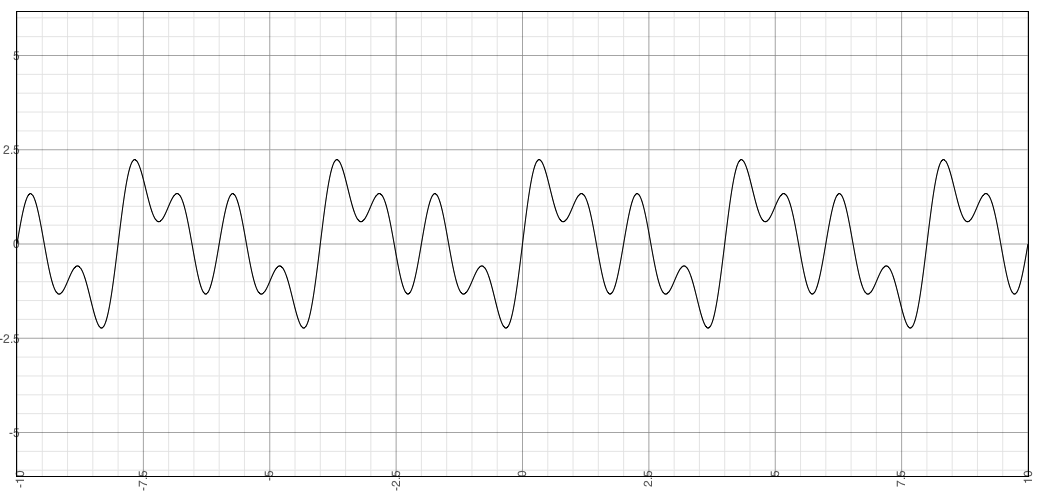
\includegraphics[width=0.8\textwidth]{figure/sin(05pix)+sin(2pix)+sin(pix)}

\begin{enumerate}
  \item Welche Frequenzen $f$ (bezogen auf den Einheitskreis) kommen im obigen Signal vor?
  \answer{
\clearpage
  $2\pi$ entspricht einer Kreisumdrehung in der Sekunde\\
  $2\pi f$ entspricht der Frequenz f (=Kreisumdrehungen pro Sekunde)\\
  $\rightarrow f_1=0.25,f_2=0.5,f_3=1 $
  }
  \item Geben sie 20 Digitalisierungswerte des abgetasteten Signals an, soda� dieses bei fortlaufender Abtastung rekonstruiert werden kann. Achten sie dabei darauf, nicht zu viele, unnotwendige Abtastwerte zu konstruieren.
\answer{
\clearpage
  Abtastfrequenz: $f_{abtast}>2*f_{max}=2*1 Hz$\\
  $sin(2\pi f_1 \mathbf{x})+sin(2\pi f_2 \mathbf{x})+sin(2\pi f_3 \mathbf{x})$, d.h. X-Achse ist
  in Sekunde\\
  Abtastung, mind. mit 2 Hz, d.h. 2 mal pro Sekunde. Der Einfachheit halber wird das Beispiel mit 4 mal pro Sekunde abgetastet (2.1 w�rde aber auch gen�gen).
  }
  \item Nehmen sie an, Ihnen stehen nur 3 Bit zur Speicherung eines Abtastwertes zu Verf�gung. Wie sieht das digitalisierte Signal aus? 
  \answer{
\clearpage
  3 Bit bedeutet 8 unterschiedliche Zust�nde, d.h. 4 in positiver und negativer Achse.
  Bei linearer Quantisierung stehen $\frac{4.9}{7}=0.7$ pro Quantisierungsstufe zu Verf�gung (1 Bit kodiert den Beginn)\\
  \bsfigure[scale=0.5]{figure/sin(05pix)+sin(2pix)+sin(pix)_lsg}
  \bsfigure[scale=0.5]{figure/sin(05pix)+sin(2pix)+sin(pix)_lsg2}
  }
  \item Gen�gen die 3-Bit zur vollst�ndigen Rekonstruktion des Signals?
  \answer{
\clearpage
  Nein. Bei der Quantsieriung erf�hrt die Digitalisierung immer einen Verlust.
  }   

  \item Wodurch unterscheidet sich die Funktion 
   $$f_{neu}(x)=sin(2\pi
    f_1 x+\pi/3)+sin(2\pi f_2 x+\pi/3)+sin(2\pi f_3
    x+7\pi/3)$$ vom Ursprungssignal $f(x)$.
   \answer{durch einen um $\pi/3$ fr\"uheren Start. Ansonsten ist das
     Signal identisch} 
\end{enumerate}

\end{exercise}


%%% Local Variables: 
%%% mode: latex
%%% TeX-master: "exercise-de-digitalisierung"
%%% End: 
